\documentclass[11pt]{article}

\usepackage[margin=1in]{geometry}
\usepackage{setspace}
\onehalfspacing
\usepackage{graphicx}
\graphicspath{report_images/}
\usepackage{appendix}
\usepackage{listings}
\usepackage{float}
\usepackage{multirow}
\usepackage{amsthm}
% The next three lines make the table and figure numbers also include section number
\usepackage{chngcntr}
\counterwithin{table}{section}
\counterwithin{figure}{section}
% Needed to make titling page without a page number
\usepackage{titling}

% DOCUMENT INFORMATION =================================================
\font\titleFont=cmr12 at 11pt
\title {{\titleFont ECEN 424: Advanced Digital Design\\ North Carolina Agricultural and Technical State University \\ Department of Electrical and Computer Engineering}} % Declare Title
\author{\titleFont Prepared by: Chris Cannon} % Declare authors
\date{\titleFont 2018-10-10}
% ======================================================================

\begin{document}

\begin{titlingpage}
\maketitle
\begin{center}
	Project 1 Specification \\ Rev. 0.2.0
\end{center}
\end{titlingpage}

\section{System Overview}
This system will be a VHDL-based digital lock that must be implemented on the Digilent Basys3 FPGA. The lock will take a 6-digit code, entered via a standard USB numeric keyboard. The code must be re-programmable. The system must notify a user of an incorrect password and must lock permanently after 3 incorrect attempts.

\section{Modules}

\subsection{Module Overview}

The system should include the following modules

\begin{table}[H]
\begin{tabular}{| p{5cm} | p{10.5cm} |}
	\hline
	Module & Description \\ \hline
	main & Main finite state machine and top-level module. \\ \hline
	code\textunderscore timeout\textunderscore timer & Counts to 20 seconds, after which it will notify the main so that the code can be cleared. \\ \hline
	set\textunderscore timeout\textunderscore timer & Counts to 10 seconds, after which it will notify the main so that the set state can be exited \\ \hline
	open\textunderscore timeout\textunderscore timer & Counts to 15 seconds, after which it will notify the main to lock the system \\ \hline
	display\textunderscore timeout\textunderscore timer & Counts to 5 seconds, after which it will notify the display-controller so that the display will be cleared \\ \hline
	clock\textunderscore divider & Divides the clock signal to 4 Hz for the input module to prevent accidental double keystrokes \\ \hline
	input\textunderscore controller & Interprets the keystrokes from the USB keyboard and passes the appropriate command to the main\\ \hline
	output\textunderscore controller & Interprets the command from main and displays the appropriate message on the 7-segment display and LED \\ \hline
\end{tabular}
\end{table}

\subsection{main}

\subsection{Overview}

The main module is the finite state machine that is the top-level component of the system.

\subsubsection{Inputs}

\begin{table}[H]
\begin{tabular}{| p{2.5cm} | p{6cm} | p{6cm} |}
	\hline
	Input Name & Data Type & Description \\ \hline
	cmd & std\textunderscore logic\textunderscore vector(3 downto 0) & Input command from the input\textunderscore controller module. \\ \hline
	code\textunderscore timeout & std\textunderscore logic & Indicates when the code entry has timed out. \\ \hline
	set\textunderscore timeout & std\textunderscore logic & Indicates when the set function has timed out. \\ \hline
	open\textunderscore timeout & std\textunderscore logic & Indicates when the lock should close. \\ \hline
	clk & std\textunderscore logic & Board clock signal \\ \hline
\end{tabular}
\end{table}

\subsubsection{Outputs}

\begin{table}[H]
\begin{tabular}{| p{2.5cm} | p{6cm} | p{6cm} |}
	\hline
	Output Name & Data Type & Description \\ \hline
	enable\textunderscore code & std\textunderscore logic & Activates the code\textunderscore timeout\textunderscore timer module. \\ \hline
	reset\textunderscore code & std\textunderscore logic & Restarts the code\textunderscore timeout\textunderscore timer module. \\ \hline
	enable\textunderscore set & std\textunderscore logic & Activates the set\textunderscore timeout\textunderscore timer module. \\ \hline
	reset\textunderscore set & std\textunderscore logic & Restarts the set\textunderscore timeout\textunderscore timer module. \\ \hline
	enable\textunderscore open & std\textunderscore logic & Activates the open\textunderscore timeout\textunderscore timer module. \\ \hline
	reset\textunderscore open & std\textunderscore logic & Restarts the open\textunderscore timeout\textunderscore timer module. \\ \hline
	display\textunderscore cmd & std\textunderscore logic\textunderscore vector(3 downto 0) & Binary encoded message for the output\textunderscore controller module. \\ \hline
\end{tabular}
\end{table}

\subsection{code\textunderscore timeout\textunderscore timer}

\subsubsection{Inputs}

\begin{table}[H]
\begin{tabular}{| p{2.5cm} | p{6cm} | p{6cm} |}
	\hline
	Input Name & Data Type & Description \\ \hline
	enable & std\textunderscore logic & Activates the code\textunderscore timeout\textunderscore timer module. \\ \hline
	reset & std\textunderscore logic & Restarts the code\textunderscore timeout\textunderscore timer module. \\ \hline
	clk & std\textunderscore logic & Board clock signal \\ \hline
\end{tabular}
\end{table}

\subsubsection{Outputs}

\begin{table}[H]
\begin{tabular}{| p{2.5cm} | p{6cm} | p{6cm} |}
	\hline
	Output Name & Data Type & Description \\ \hline
	done & std\textunderscore logic & Indicates when the code entry has timed out. \\ \hline
\end{tabular}
\end{table}

\subsection{set\textunderscore timeout\textunderscore timer}

\subsubsection{Inputs}

\begin{table}[H]
\begin{tabular}{| p{2.5cm} | p{6cm} | p{6cm} |}
	\hline
	Input Name & Data Type & Description \\ \hline
	enable & std\textunderscore logic & Activates the set\textunderscore timeout\textunderscore timer module. \\ \hline
	reset & std\textunderscore logic & Restarts the set\textunderscore timeout\textunderscore timer module. \\ \hline
	clk & std\textunderscore logic & Board clock signal \\ \hline
\end{tabular}
\end{table}

\subsubsection{Outputs}

\begin{table}[H]
\begin{tabular}{| p{2.5cm} | p{6cm} | p{6cm} |}
	\hline
	Output Name & Data Type & Description \\ \hline
	done & std\textunderscore logic & Indicates when the set operation has timed out. \\ \hline
\end{tabular}
\end{table}

\subsection{open\textunderscore timeout\textunderscore timer}

\subsubsection{Inputs}

\begin{table}[H]
\begin{tabular}{| p{2.5cm} | p{6cm} | p{6cm} |}
	\hline
	Input Name & Data Type & Description \\ \hline
	enable & std\textunderscore logic & Activates the open\textunderscore timeout\textunderscore timer module. \\ \hline
	reset & std\textunderscore logic & Restarts the open\textunderscore timeout\textunderscore timer module. \\ \hline
	clk & std\textunderscore logic & Board clock signal \\ \hline
\end{tabular}
\end{table}

\subsubsection{Outputs}

\begin{table}[H]
\begin{tabular}{| p{2.5cm} | p{6cm} | p{6cm} |}
	\hline
	Output Name & Data Type & Description \\ \hline
	done & std\textunderscore logic & Indicates when the open state has timed out. \\ \hline
\end{tabular}
\end{table}

\subsection{display\textunderscore timeout\textunderscore timer}

\subsubsection{Inputs}

\begin{table}[H]
\begin{tabular}{| p{2.5cm} | p{6cm} | p{6cm} |}
	\hline
	Input Name & Data Type & Description \\ \hline
	enable & std\textunderscore logic & Activates the display\textunderscore timeout\textunderscore timer module. \\ \hline
	reset & std\textunderscore logic & Restarts the display\textunderscore timeout\textunderscore timer module. \\ \hline
	clk & std\textunderscore logic & Board clock signal \\ \hline
\end{tabular}
\end{table}

\subsubsection{Outputs}

\begin{table}[H]
\begin{tabular}{| p{2.5cm} | p{6cm} | p{6cm} |}
	\hline
	Output Name & Data Type & Description \\ \hline
	done & std\textunderscore logic & Indicates when the display shown has timed out. \\ \hline
\end{tabular}
\end{table}

\subsection{clock\textunderscore divider}

\subsubsection{Inputs}

\begin{table}[H]
\begin{tabular}{| p{2.5cm} | p{6cm} | p{6cm} |}
	\hline
	Input Name & Data Type & Description \\ \hline
	clk & std\textunderscore logic & Board clock signal \\ \hline
\end{tabular}
\end{table}

\subsubsection{Outputs}

\begin{table}[H]
\begin{tabular}{| p{2.5cm} | p{6cm} | p{6cm} |}
	\hline
	Output Name & Data Type & Description \\ \hline
	button\textunderscore clock & std\textunderscore logic & Reduced 4 Hz clock signal for the input\textunderscore controller module. \\ \hline
\end{tabular}
\end{table}

\subsection{input\textunderscore controller}

\subsubsection{Inputs}

\begin{table}[H]
\begin{tabular}{| p{2.5cm} | p{6cm} | p{6cm} |}
	\hline
	Input Name & Data Type & Description \\ \hline
	PS2Data & variable & Data stream from the USB keyboard. \\ \hline
	button\textunderscore clock & std\textunderscore logic & Reduced 4 Hz clock signal for reading from the keyboard \\ \hline
\end{tabular}
\end{table}

\subsubsection{Outputs}

\begin{table}[H]
\begin{tabular}{| p{2.5cm} | p{6cm} | p{6cm} |}
	\hline
	Output Name & Data Type & Description \\ \hline
	cmd & std\textunderscore logic\textunderscore vector(3 downto 0) & Command-code to for main method based on the input received. \\ \hline
\end{tabular}
\end{table}

\subsection{output\textunderscore controller}

\subsubsection{Inputs}

\begin{table}[H]
\begin{tabular}{| p{2.5cm} | p{6cm} | p{6cm} |}
	\hline
	Input Name & Data Type & Description \\ \hline
	display & std\textunderscore logic\textunderscore vector(3 downto 0) & Binary encoded message to display on 7-segment display \\ \hline
	timeout & std\textunderscore logic & Notifies the controller that the maximum display time has been reached and it should clear any message except "OPEN" \\ \hline
	clk & std\textunderscore logic & Board clock signal \\ \hline
\end{tabular}
\end{table}

\subsubsection{Outputs}

\begin{table}[H]
\begin{tabular}{| p{2.5cm} | p{6cm} | p{6cm} |}
	\hline
	Output Name & Data Type & Description \\ \hline
	enable & std\textunderscore logic & Activates the set\textunderscore timeout\textunderscore timer module. \\ \hline
	reset & std\textunderscore logic & Restarts the set\textunderscore timeout\textunderscore timer module. \\ \hline
	led & std\textunderscore logic & Displays if the system is in "lockdown" mode. \\ \hline
	seven\textunderscore seg &  std\textunderscore logic\textunderscore vector(11 downto 0) & Output for the message to be displayed on the seven-segment display. \\ \hline
\end{tabular}
\end{table}

\subsection{System Diagrams}

\begin{figure}[H]
\begin{center}
	\includegraphics[width=\textwidth]{./images/level0.png}
	\caption{\label{fig:level0}Level 0 System Diagram}
\end{center}
\end{figure}

\begin{figure}[H]
\begin{center}
	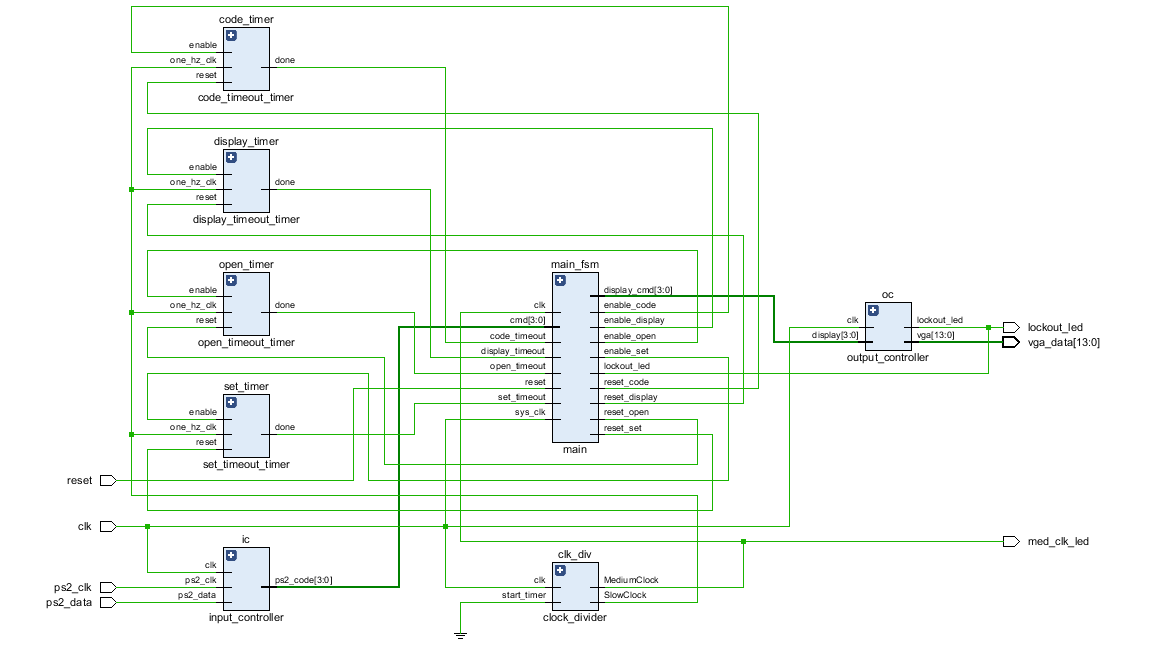
\includegraphics[width=\textwidth]{./images/level1.png}
	\caption{\label{fig:level1}Level 1 System Diagram}
\end{center}
\end{figure}

\section{Functional Specification}

\subsection{Initial Setup}

Initially, the system will have no code programmed. The user may program a code by pressing '+' to enter set mode. The user should then enter a 6-digit numeric code on the keypad and then press the '+' button again. This will exit set mode and save the code.

If the user enters more or less than 6 digits, or any non-numeric characters, the '+' key will cause the currently entered code to be cleared so the user may start setting again. If the code is cleared in this way, the 7-segment display should read "clr".

\subsection{Unlocking the Lock}

The keypad will be read every 0.25 seconds. The user should enter 6 numeric characters. As each character is entered,  it will be displayed on the least significant 7-segment display. After 6 characters are read, the system will display "0000" on the 7-segment displays if the correct code was entered, and "Err" if it was not.

The lock will remain unlocked for 15 seconds, and then the message will disappear and the system will be locked.

\subsection{Changing the Code}

To change the code after initial setup, the user must first enter the code. Then, while "OPEN" is displayed, press the '+' button to enter set mode.

Then, enter a 6-digit numeric code on the keypad and press the '+' button again. This will exit set mode and save the code.

If the user enters more or less than 6 digits, or any non-numeric characters, the '+' key will cause the currently entered code to be cleared so the user may start again. If the code is cleared in this way, the 7-segment display should read "clr".

\subsection{Display Timeout}

All messages on the 7-segment display, except for the "OPEN" message, will disappear after 2 seconds, or until a new character is entered, whichever comes first.

\subsection{Code Input Timeout}

If less then 6 digits are entered, they will be cleared after 20 seconds of no input from the user.

\subsection{Lockdown Mode}

If the incorrect code is entered 3 time, the system will enter lockdown mode. This will activate an LED indicator and the system will not unlock until its power is cycled.

\section{Development Milestones}

The following schedule is an estimated timeline for completion of the digital lock. And item containing the term "submit" is a deadline.

\begin{itemize}
	\item 2018-10-10 Submit specification rev 0.1.0
	\item 2018-10-17 Complete specification rev. 0.2.0
	\begin{itemize}
		\item Submit block diagram and timeline revisions
	\end{itemize}
	\item 2018-10-17 Complete output controller with tests
	\begin{itemize}
		\item Submit output controller as major component
	\end{itemize}
	\item 2018-10-19 Complete input controller with tests
	\item 2018-10-20 Complete clock divider with tests
	\item 2018-10-22 Complete timer components with tests
	\begin{itemize}
		\item Submit input controller, clock divider, code timer, open timer, and display timer components
	\end{itemize}
	\item 2018-10-24 Complete main component with tests
	\item 2018-10-29 Complete output controller component with tests
	\begin{itemize}
		\item Submit main component and output controller components with tests
	\end{itemize}
	\item 2018-10-31 Complete final revisions of system
	\item 2018-11-02 Draft presentation and report
	\item 2018-11-05 Submit and present final report and presentation
\end{itemize}

\end{document}